\documentclass[11pt]{article}
\usepackage{../EllioStyle}
\usepackage{listings}
\usepackage{mathtools}

\definecolor{codegreen}{rgb}{0,0.6,0}
\definecolor{codegray}{rgb}{0.5,0.5,0.5}
\definecolor{codepurple}{rgb}{0.58,0,0.82}
\definecolor{backcolour}{rgb}{0.95,0.95,0.92}

\graphicspath{ {imgs/} }

\title{Homework 6}
\author{Elliott Pryor}
\date{16 November 2023}

\rhead{Homework 6}
\lhead{Elliott Pryor}

\begin{document}
\maketitle

\problem{1}
Find the transfer function for the block diagrams:
\begin{figure}[h] 
    \centering
    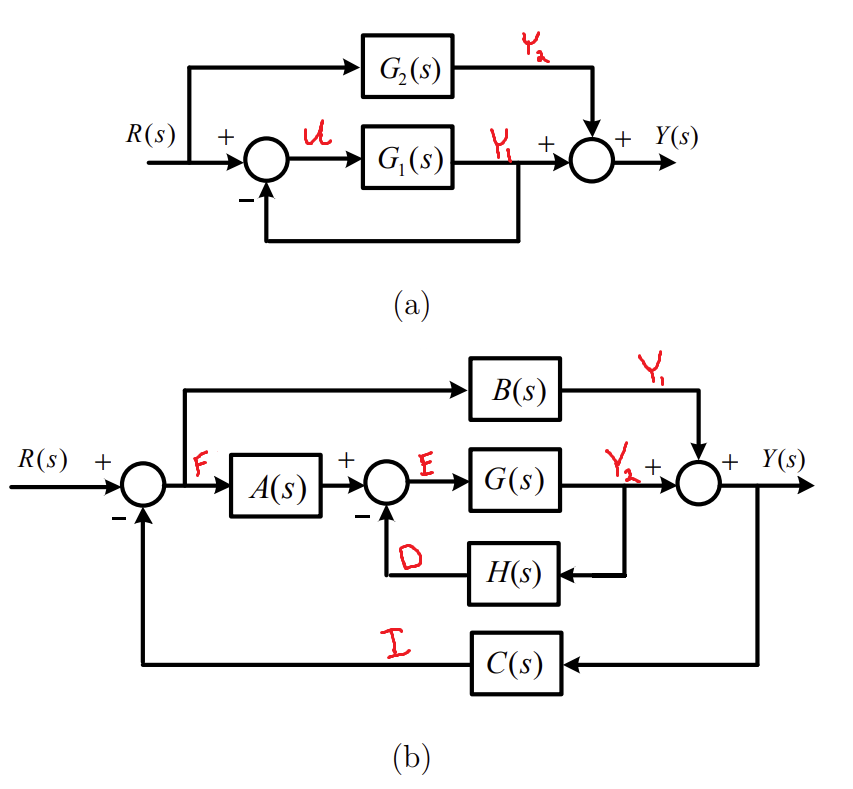
\includegraphics[width=0.55 \linewidth]{prob1}
    \caption{Problem 1}
    \label{fig:p1}
\end{figure}

\soln

\begin{enumerate}[a)]
    \item $Y(s) = Y_1(s) + Y_2(s) = G_1(s) U(s) + G_2(s)R(s)$,\\
    $U(s) = R(s) - G_1(s)U(s) \implies (1 + G_1(s))U(s) = R(s) \implies U(s) = \frac{R(s)}{1 + G_1(s)}$ \\
    So, $Y(s) = \left[\frac{G_1(s)}{1 + G_1(s)} + G_2(s)\right] R(s)$
    \item So we are going to start in the inside and go outside.
    \begin{align*}
        Y_2(s) &= G(s)E(s) \\
        E(s) &= A(s)F(s) - H(s)Y_2(s)\\
        Y_2(s) &= G(s)A(s)F(s) - G(s)H(s)Y_2(s)\\
        Y_2(s) &= \frac{G(s)A(s)F(s)}{1 + G(s)H(s)}\\
    \end{align*}
    Now this gives us the middle component. Now we can use this to find the outer component.
    $Y_1(s) = B(s)F(s)$ is easy. And our last equation: $F(s) = R(s) - C(s) Y(s)$ will bring everything together.
    We know \begin{align*}
        Y(s) &= Y_1(s) + Y_2(s) \\ 
        &= B(s)F(s) + \frac{G(s)A(s)F(s)}{1 + G(s)H(s)} \\ 
        &= \left[B(s) + \frac{G(s)A(s)}{1 + G(s)H(s)} \right] F(s) \\
        &= \left[B(s) + \frac{G(s)A(s)}{1 + G(s)H(s)} \right] \left[R(s) - C(s) Y(s) \right] \\
        Y(s) &= \left[B(s) + \frac{G(s)A(s)}{1 + G(s)H(s)} \right] R(s) - \\
        & \quad\quad \left[B(s)C(s) + \frac{G(s)A(s)C(s)}{1 + G(s)H(s)} \right]  Y(s)\\
        Y(s) \left[1 + B(s) C(s) + \frac{G(s)A(s)C(s)}{1 + G(s)H(s)} \right] &= \left[B(s) + \frac{G(s)A(s)}{1 + G(s)H(s)} \right] R(s) \\
        Y(s) &= \frac{\left[B(s) + \frac{G(s)A(s)}{1 + G(s)H(s)} \right]}{\left[1 + B(s) C(s) + \frac{G(s)A(s)C(s)}{1 + G(s)H(s)} \right]} R(s) \\
    \end{align*}
\end{enumerate}



\problem{2}
Determine the time constant of the system:
\begin{figure}[h] 
    \centering
    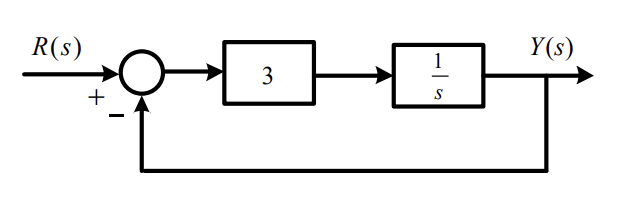
\includegraphics[width=0.55 \linewidth]{prob2}
    \caption{Problem 2}
    \label{fig:p2}
\end{figure}

\soln

First we need to write the transfer function for the system. We can do this by using the block diagram.
$Y(s) = \frac{3}{s}U(s)$, and $U(s) = R(s) - Y(s)$, so \\
$Y(s) = \frac{3}{s} \left[R(s) - Y(s) \right] \implies 
Y(s) = \frac{1}{1 + 3/s}R(s) = \frac{s}{s + 3}R(s)$.
We want the response to a unit step, so $R(s) = \frac{1}{s}$, so $Y(s) = \frac{1}{s+3}$,
thus $y(t) = e^{-3t}$, so our time constant is $\frac{1}{3}$


\problem{3}
Specify the gain K
of the proportional controller so that the output $y(t)$ has an overshoot of no more then 10\%
in response to a unit step

\begin{figure}[h] 
    \centering
    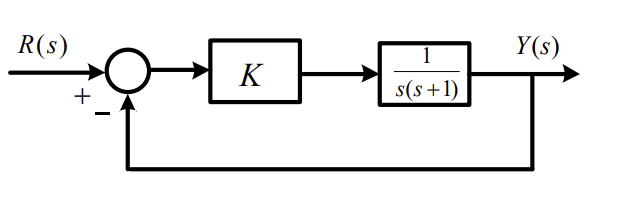
\includegraphics[width=0.55 \linewidth]{prob3}
    \caption{Problem 3}
    \label{fig:p3}
\end{figure}

\soln

First, we go for the transfer function:
$Y(s) = K G(s) U(s)$, and $U(s) = R(s) - Y(s)$, so $Y(s) = \frac{K G(s)}{1 + G(s)}R(s)$.
\begin{align*}
    Y(s) &= \frac{K G(s)}{1 + G(s)} R(s)\\
    &= \frac{K \frac{1}{s(s+1)}}{1 + \frac{1}{s(s+1)}} R(s)\\
    &= \frac{K \frac{1}{s(s+1)}}{\frac{s(s+1) + 1}{s(s+1)}} R(s)\\
    &= \frac{K}{s^2 + s + 1} R(s)\\
\end{align*}
We recognize the standard form of a second order system, so we can use the standard formula for the overshoot.
$G(s) = \frac{\omega_n^2}{s^2 + 2 \xi \omega_n s + \omega_n^2}$,
so in our case $\omega_n = \sqrt{K}$, so $\xi = \frac{1}{2 \sqrt{K}}$,\\
then \begin{align*}
    M_p &= \exp\left(\frac{-\pi \xi}{\sqrt{1 - \xi^2}}\right) \\
    &= \exp\left(\frac{-\pi \frac{1}{2 \sqrt{K}}}{\sqrt{1 - \frac{1}{4 K}}}\right) \\
    &= \exp\left(\frac{-\pi \frac{1}{2 \sqrt{K}}}{\frac{\sqrt{4K - 1}}{2 \sqrt{K}}}\right) \\
    &= \exp\left(\frac{-\pi}{\sqrt{4K - 1}}\right) \\
\end{align*}

We want $M_p \leq 0.1$, so we solve:
\begin{align*}
    0.1 \leq \exp\left(\frac{-\pi}{\sqrt{4K - 1}}\right) \\
    \ln(0.1) \leq \frac{-\pi}{\sqrt{4K - 1}} \\
    \ln(0.1) \sqrt{4K - 1} \leq -\pi \\
    \sqrt{4K - 1} \geq -\frac{\pi}{\ln(0.1)} \\
    4K - 1 \geq \frac{\pi^2}{\ln(0.1)^2} \\
    K \geq \frac{\pi^2}{4 \ln(0.1)^2} + \frac{1}{4} \\
    K \geq 0.715381 \\
\end{align*}

So pick $K = 0.75$

\problem{4}

Consider the system
\begin{figure}[h] 
    \centering
    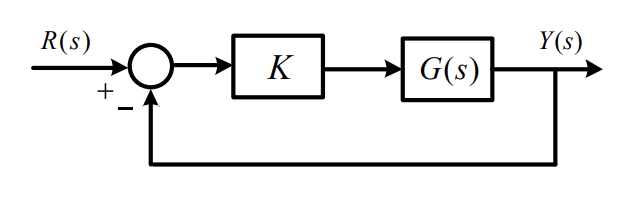
\includegraphics[width=0.55 \linewidth]{prob4}
    \caption{Problem 4}
    \label{fig:p4}
\end{figure}

with \begin{enumerate}[a)]
    \item $KG(s) = \frac{4(s+2)}{s(s^3+2s^2+3s+4)}$
    \item $KG(s) = \frac{2(s+4)}{s^2(s+1)}$
\end{enumerate}

Use Routh's stability criterion to determine whether the each of the resulting closed-loop
system will be asymptotically stable.

\soln

with \begin{enumerate}[a)]
    \item $KG(s) = \frac{4(s+2)}{s(s^3+2s^2+3s+4)}$
    We multiply this out to get: $\frac{4s+8}{s^4+2s^3+3s^2+4s}$, and then we can write the Routh table:
    \begin{center}
        \begin{tabular}{c|c c}
            $s^4$ & 1 & 3 \\
            $s^3$ & 2 & 4 \\
            $s^2$ & -$\frac{4-6}{2}=1$ & 0 \\
            $s^1$ & 4 & * \\
            $s^0$ & 0 & * \\
        \end{tabular}
    \end{center}
    Which has no sign changes, so there are no poles with a positive real part. So the system is marginally stable.
        
    \item $KG(s) = \frac{2(s+4)}{s^2(s+1)} = \frac{2s + 8}{s^3 + s^2}$. We can write the Routh table:
    \begin{center}
        \begin{tabular}{c|c c}
            $s^3$ & 1 & 0 \\
            $s^2$ & 1 & 0 \\
            $s^1$ & $0 \to 2$ & * \\
            $s^0$ & $\frac{0}{-2} = 0$ & * \\
        \end{tabular}
    \end{center}
    for the $s^1$ row of zeros: $s^2 + 4 \to 2s + 0$.
    This also has no sign changes, but the last value is zero. So it is marginally stable.
        
    
\end{enumerate}





\problem{5}
Using Routh's stability criterion to determine how many roots with positive
real parts the following equations have: 

\begin{enumerate}[a)]
    \item $s^4 + 8s^3 + 32s^2 + 80s + 100 = 0$
    \item $s^5 + 10s^4 + 30s^3 + 80s^2 + 344s + 480 = 0$
\end{enumerate}

\soln

\begin{enumerate}[a)]
    \item We write the Routh table:
    \begin{center}
        \begin{tabular}{c|c c c}
            $s^4$ & 1 & 32 & 100\\
            $s^3$ & 8 & 80 & 0\\
            $s^2$ & 22 & 100 & 0\\
            $s^1$ & $\frac{960}{22}$ & * & *\\
            $s^0$ & $\frac{960*100}{22} * \frac{22}{960} = 100$
        \end{tabular}
    \end{center}
    So no roots have positive real parts. 

    \item We write the Routh table:
    \begin{center}
        \begin{tabular}{c|c c c}
            $s^5$ & 1 & 30 & 344\\
            $s^4$ & 10 & 80 & 480\\
            $s^3$ & 22 & 296 & 0\\
            $s^2$ & $-\frac{600}{11}$ & 480 & *\\
            $s^1$ & $-(22*480+\frac{600}{11}*296)\frac{-11}{600} = \frac{968}{5} + 296$ & * & *\\
            $s^0$ & 480 & * & *\\
        \end{tabular}
    \end{center}
    There are two sign changes, so two roots with positive real parts.
\end{enumerate}



\problem{6}

Consider the closed-loop system:
\begin{figure}[h] 
    \centering
    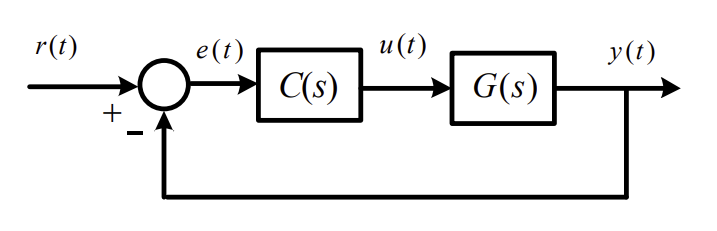
\includegraphics[width=0.55 \linewidth]{prob6}
    \caption{Problem 6}
    \label{fig:p6}
\end{figure}

$G(s) = \frac{1}{s^2}$, and $C(s) = \frac{10(s+2)}{s+5}$.

Find the system type and determine the steady state tracking errors for:

\begin{enumerate}[a)]
    \item $r(t) = 1(t)$
    \item $r(t) = t1(t)$
    \item $r(t) = 1/2 t^2 1(t)$
\end{enumerate}

\soln

So $L(s) = G(s)C(s) = \frac{10(s+2)}{s^2(s+5)}$. So it is a type 2 system with $L_0 = \frac{10(s+2)}{s+5}$,
we evaluate this at $s = 0$ to get $L_0 = 4$. This is $K_a$. So the steady state error is:

\begin{enumerate}[a)]
    \item $r(t) = 1(t) \implies 0$
    \item $r(t) = t1(t) \implies 0$
    \item $r(t) = 1/2 t^2 1(t) \implies 1/4$
\end{enumerate}


\problem{7}
Sketch the Nyquist plot for an open-loop system with transfer function:
\begin{enumerate}[a)]
    \item $G(s) = \frac{1}{s^2}$
    \item $G(s) = \frac{1}{s^2 + 4}$
\end{enumerate}

\soln

\begin{figure}[h] 
    \centering
    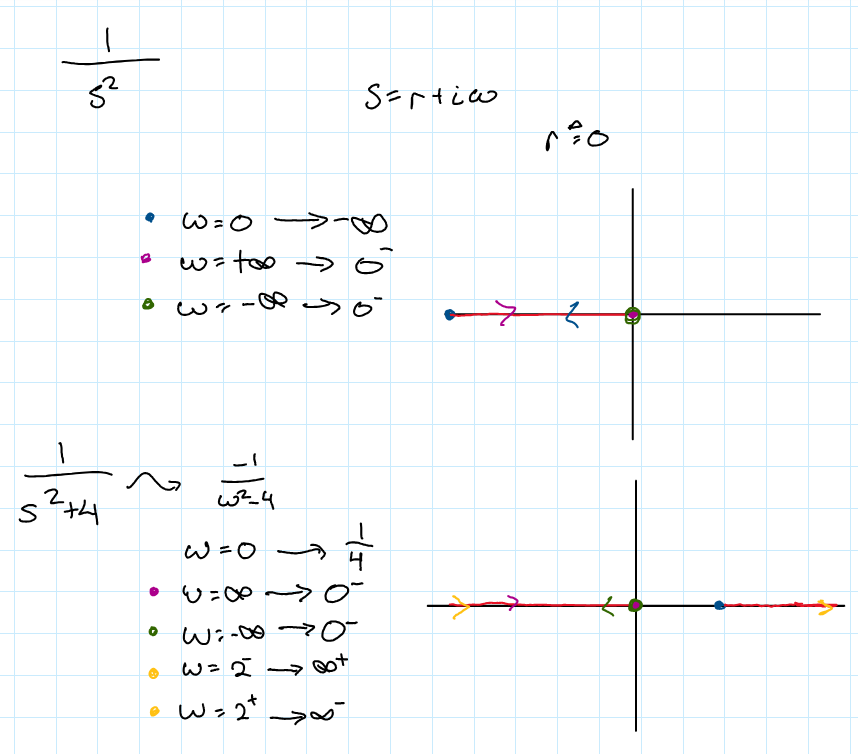
\includegraphics[width=0.55 \linewidth]{11-20-p7.png}
    \caption{}
    \label{fig:}
\end{figure}

\begin{enumerate}
    \item First we solve for $G(i\omega)$:
    \begin{align*}
        G(i\omega) &= \frac{1}{(i\omega)^2} \\
        &= \frac{1}{- \omega^2} \\
        &= -\frac{1}{\omega^2} \\
    \end{align*}
    So this is just the negative real line.

    \item First we solve for $G(i\omega)$:
    \begin{align*}
        G(i\omega) &= \frac{1}{(i\omega)^2 + 4} \\
        &= \frac{1}{- \omega^2 + 4} \\
        &= -\frac{1}{\omega^2 - 4} \\
    \end{align*}
    So this starts at $1/4$, goes to $+ \infty$, then teleports to $-\infty$ and goes to zero before turning around.

\end{enumerate}







\problem{8}
Consider the system with loop gain
$$
L(s) = KG(s) = \frac{K(s+2)}{s+10}
$$
Use Matlab command nyquist to plot nyquist plot for $G(s)$, and based
on the nyquist plot, determine the range of $K$ for which the closed-loop system is asymptotically stable
\soln

\begin{figure}[h] 
    \centering
    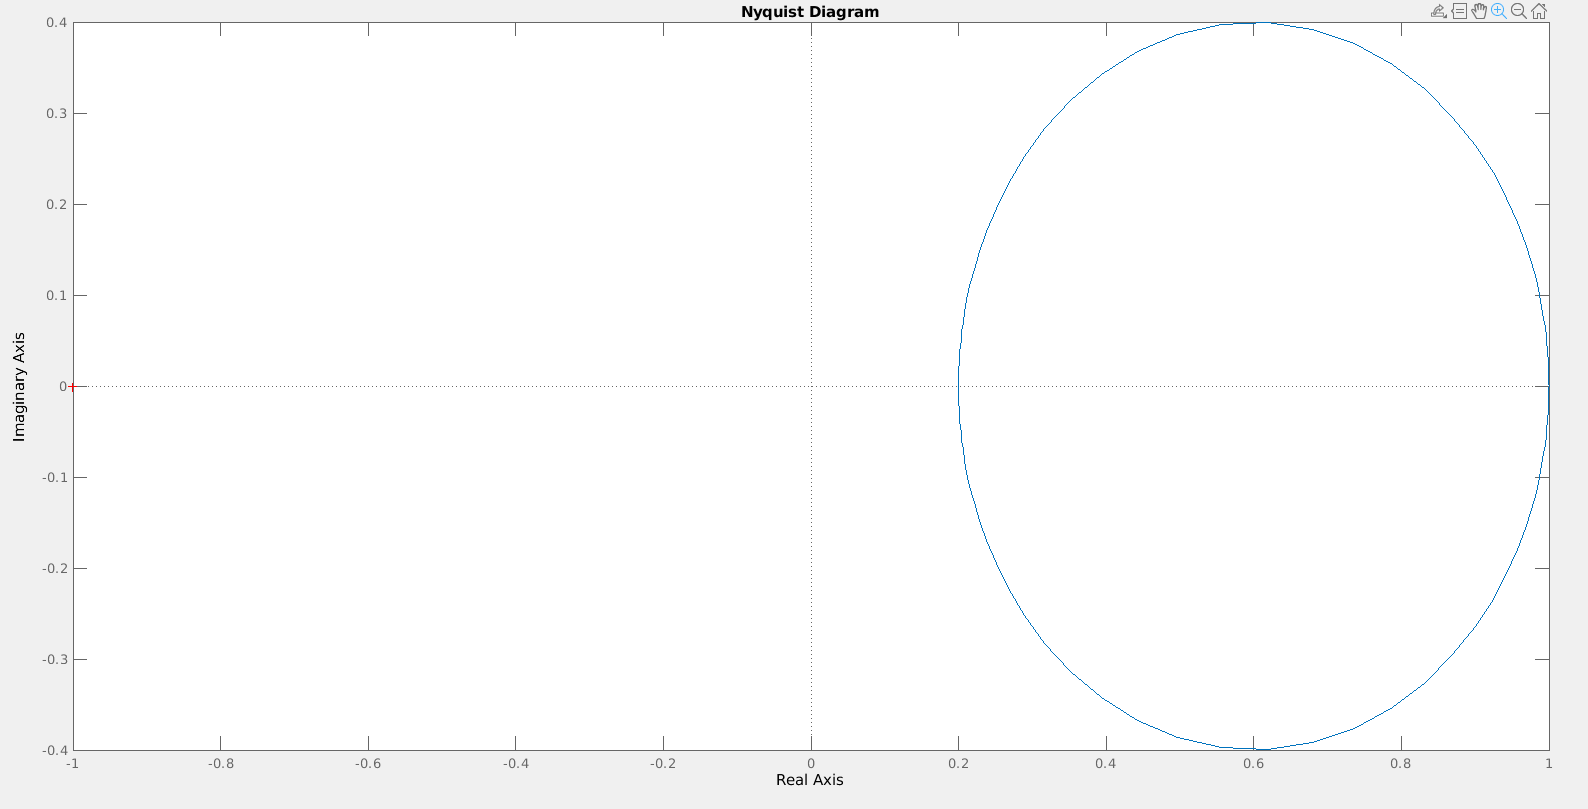
\includegraphics[width=0.55 \linewidth]{11-20-nyquist.png}
    \caption{}
    \label{fig:}
\end{figure}

We also solve for 
\begin{align*}
    L(i\omega) &= \frac{K(i\omega + 2)}{i\omega + 10} \\
    &= \frac{K(i\omega + 2)(-i\omega + 10)}{(i\omega + 10)(-i\omega + 10)} \\
    &= \frac{K(\omega^2 + 8i\omega + 20)}{\omega^2 + 100} \\
    &= K \frac{\omega^2 + 20}{\omega^2 + 100}  + iK \frac{8\omega}{\omega^2 + 100} \\\\
\end{align*}

So we can see that the real part is always positive, thus the system can never encircle -1,
so the system is always asymptotically stable.

\problem{9}
Is the following system controllable? Observable?

\begin{align*}
    \dot{x} &= \begin{bmatrix}
        0 & 1 \\ -1 & -1
    \end{bmatrix} x + \begin{pmatrix}
        0 \\ 1
    \end{pmatrix} u \\
    y &= \begin{pmatrix}
        1 & 0
    \end{pmatrix} x
\end{align*}

\soln

For controllability, we build the controllability matrix.
$C = \begin{bmatrix}
    B & AB
\end{bmatrix}$
$AB = \begin{bmatrix}
    1 \\ -1
\end{bmatrix}$, so $C = \begin{bmatrix}
    0 & 1 \\ 1 & -1
\end{bmatrix}$
which is full rank, so it is controllable.

For observability, we build the observability matrix.
$O = \begin{bmatrix}
    C \\ CA
\end{bmatrix}$
$CA = \begin{bmatrix}
    0 & 1 \end{bmatrix}$, so $O = \begin{bmatrix}
    1 & 0 \\ 0 & 1 \end{bmatrix}$
which is full rank, so it is observable.

\end{document}